% Chapter 1

\chapter{Stages of OCR Process} % Main chapter title

\label{Chapter2} % For referencing the chapter elsewhere, use \ref{Chapter1} 

\lhead{Chapter 2. \emph{Introduction}} % This is for the header on each page - perhaps a shortened title

\section{Stages of OCR Process }
Optical Character Recognition is a complex process .To solve the problem of OCR we have chosen the following stages.
\begin{itemize}
  
  \item Preprossessing and Binarization.
  \item Line and Word Segmentation.
  \item Word recognition with CNN LSTM Neural Network.
  \item Data Preparation.
\end{itemize}


\section{Preprossessing and Binarization}
Preprocessing and Binarization is First stage of OCR process. In this stage we have corrected the skew and used ostu binarization algorithm to convert the RGB image into GrayScale by remove noise.

\section{Line and Word Segmentation}
This Stage of process segments the image into lines and further the line image are segmented into word images
\begin{figure}[h]

\includegraphics{Figures/my_tel_img.png}
\caption{A Telugu Text Image}
\end{figure}
%
\includegraphics{Figures/my_tel_img.png} \\
%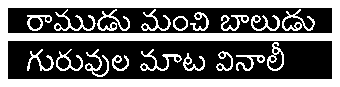
\includegraphics{Figures/merge_img.png}


